\documentclass[conference]{IEEEtran}

\usepackage{amsmath,amssymb,amsfonts}
\usepackage{graphicx}
\usepackage{textcomp}
\usepackage{booktabs}
\usepackage{multirow}
\usepackage{algorithmic}
\usepackage{algorithm}
\usepackage{hyperref}
\usepackage{xcolor}
\usepackage{array}

\begin{document}

\title{LSGNN-DualTask: A Graph Neural Network with Edge Consistency Regularization for Network Intrusion Detection}

\author{
\IEEEauthorblockN{Author One\IEEEauthorrefmark{1}, Author Two\IEEEauthorrefmark{1}, Author Three\IEEEauthorrefmark{1}}
\IEEEauthorblockA{\IEEEauthorrefmark{1}Department of Computer Science\\
University Placeholder, City, Country\\
\{author.one, author.two, author.three\}@university.edu}
}

\maketitle

\begin{abstract}
Network intrusion detection remains a critical challenge in cybersecurity, particularly when dealing with imbalanced, sparse packet-level data. In this paper, we present an end-to-end pipeline for network intrusion detection that combines extensive feature engineering from raw packet captures with graph neural network (GNN) classification. We introduce LSGNN-DualTask, a novel extension of the Local Similarity Graph Neural Network (LSGNN) that augments the standard node classification objective with an auxiliary edge consistency loss. This dual-task formulation encourages the model to learn embeddings where connected nodes of the same attack type are clustered tightly, while sharpening the boundary between normal and malicious traffic. We evaluate our approach on a real-world labeled packet capture dataset containing 76{,}500 network flows across five traffic classes with class imbalance (40:1 ratio). Experiments show that Random Forest achieves the strongest overall results (accuracy: 0.7142; macro F1: 0.6873), while among neural approaches, LSGNN-DualTask outperforms the baseline LSGNN across all metrics (accuracy: 0.6721 vs.\ 0.6538; macro F1: 0.6385 vs.\ 0.6147), with consistent gains observed across most attack classes. We also provide a systematic comparison with tabular baselines (Random Forest, MLP) and analyze the contribution of each pipeline component.
\end{abstract}

\begin{IEEEkeywords}
Graph Neural Networks, Network Intrusion Detection, Cybersecurity, Class Imbalance, Dual-Task Learning, LSGNN, Edge Consistency
\end{IEEEkeywords}

% ======================================================================
\section{Introduction}
% ======================================================================

Network intrusion detection systems (NIDS) are a cornerstone of modern cybersecurity infrastructure, tasked with identifying malicious activities from network traffic in real time~\cite{buczak2016survey}. Traditional NIDS rely on signature-based matching or manually engineered statistical features, which struggle to generalize to novel attack patterns. Machine learning approaches have shown promise in automating the detection of both known and unknown threats~\cite{ahmad2021network}, but most existing methods treat network flows as independent samples, ignoring the relational structure inherent in network communication.

Graph Neural Networks (GNNs) offer a natural framework for modeling network traffic, as communication patterns between hosts form a graph structure where nodes represent flows or hosts and edges encode communication relationships~\cite{zhou2020graph}. Recent work has demonstrated the effectiveness of GNNs for intrusion detection~\cite{lo2022graphsage_ids, chang2021gnn_nids}, as they can propagate suspicion signals across related flows and capture higher-order structural patterns that flat classifiers miss.

However, applying GNNs to cybersecurity data presents several challenges:
\begin{itemize}
    \item \textbf{Sparse raw features}: Packet-level captures often contain very few columns (IP addresses, ports, protocol, payload length), requiring extensive feature engineering to provide sufficient signal.
    \item \textbf{Severe class imbalance}: Real-world attack datasets exhibit extreme imbalance, with rare attack types comprising a small fraction of samples.
    \item \textbf{Heterophilic graph structure}: Unlike social networks, cybersecurity graphs often connect nodes of different classes (e.g., normal flows adjacent to attack flows on the same host), violating the homophily assumption of standard GNNs.
\end{itemize}

In this paper, we address these challenges with an end-to-end pipeline comprising: (1) comprehensive feature engineering from raw packet data, (2) a hybrid graph construction strategy combining feature-space similarity with communication-pattern edges, (3) SMOTE-based data augmentation for class balance, and (4) a novel dual-task GNN architecture. Our main contribution is LSGNN-DualTask, which extends the Local Similarity GNN~\cite{wu2023lsgnn} with an auxiliary edge consistency prediction objective that trains the model to recognize whether connected nodes share the same traffic type. This regularizes the learned representations to respect graph structure, yielding improved detection of attack classes.

Our contributions are summarized as follows:
\begin{enumerate}
    \item We design an end-to-end pipeline that transforms sparse packet-level data (9 raw columns) into a rich 68-dimensional feature space suitable for GNN-based classification.
    \item We propose LSGNN-DualTask, a dual-task extension that combines node classification with edge consistency prediction, providing structural regularization without architectural changes.
    \item We conduct a systematic comparison of four model families (Random Forest, MLP, LSGNN, LSGNN-DualTask) on a real-world dataset with five attack types and class imbalance.
    \item We demonstrate that the dual-task formulation improves the baseline LSGNN by +2.38\% average per-class F1, with consistent gains across most attack classes.
\end{enumerate}

% ======================================================================
\section{Related Work}
% ======================================================================

\subsection{Machine Learning for Intrusion Detection}

Machine learning has been extensively applied to network intrusion detection, spanning classical methods such as Random Forests, Support Vector Machines, and ensemble approaches~\cite{buczak2016survey}. Deep learning methods, including autoencoders, convolutional neural networks, and recurrent networks, have shown improvements on benchmark datasets such as NSL-KDD, UNSW-NB15, and CICIDS~\cite{ahmad2021network, ferrag2020deep}. However, most methods treat each network flow independently, discarding the relational structure of network communication.

\subsection{Graph Neural Networks for Cybersecurity}

GNNs have emerged as a promising paradigm for cybersecurity tasks due to their ability to model relational data. Lo et al.~\cite{lo2022graphsage_ids} applied GraphSAGE to intrusion detection by constructing flow-level graphs and demonstrated improvements over tabular methods. Chang et al.~\cite{chang2021gnn_nids} proposed a GNN-based NIDS that captures host-level communication patterns. Pujol-Perich et al.~\cite{pujol2022unveiling} used GNNs for botnet detection by modeling network topologies. These works highlight the potential of graph-based approaches but typically rely on standard message-passing architectures (GCN, GAT, GraphSAGE) that assume homophilic graph structure.

\subsection{Handling Heterophily in GNNs}

Standard GNNs perform poorly on heterophilic graphs where connected nodes often have different labels~\cite{zhu2020beyond}. Several architectures have been proposed to address this, including H2GCN~\cite{zhu2020beyond}, LINKX~\cite{lim2021large}, and LSGNN~\cite{wu2023lsgnn}. LSGNN introduces local similarity-weighted message passing that adaptively attends to or suppresses neighbor messages based on feature similarity, making it well-suited for cybersecurity graphs where normal and attack flows coexist on the same hosts.

\subsection{Multi-Task and Auxiliary Losses for GNNs}

Multi-task learning has been used to improve GNN representations by providing additional supervisory signals. Self-supervised objectives such as link prediction, graph contrastive learning, and node attribute reconstruction have been shown to regularize GNN training and improve downstream classification~\cite{you2020graph, velickovic2019deep}. Our edge consistency loss is related to link prediction but differs in that it predicts label agreement rather than edge existence, providing a more directly task-relevant auxiliary objective.

% ======================================================================
\section{Proposed Method}
% ======================================================================

We present our complete pipeline for GNN-based network intrusion detection. The system architecture is illustrated in Fig.~\ref{fig:pipeline}.

\begin{figure}[t]
    \centering
    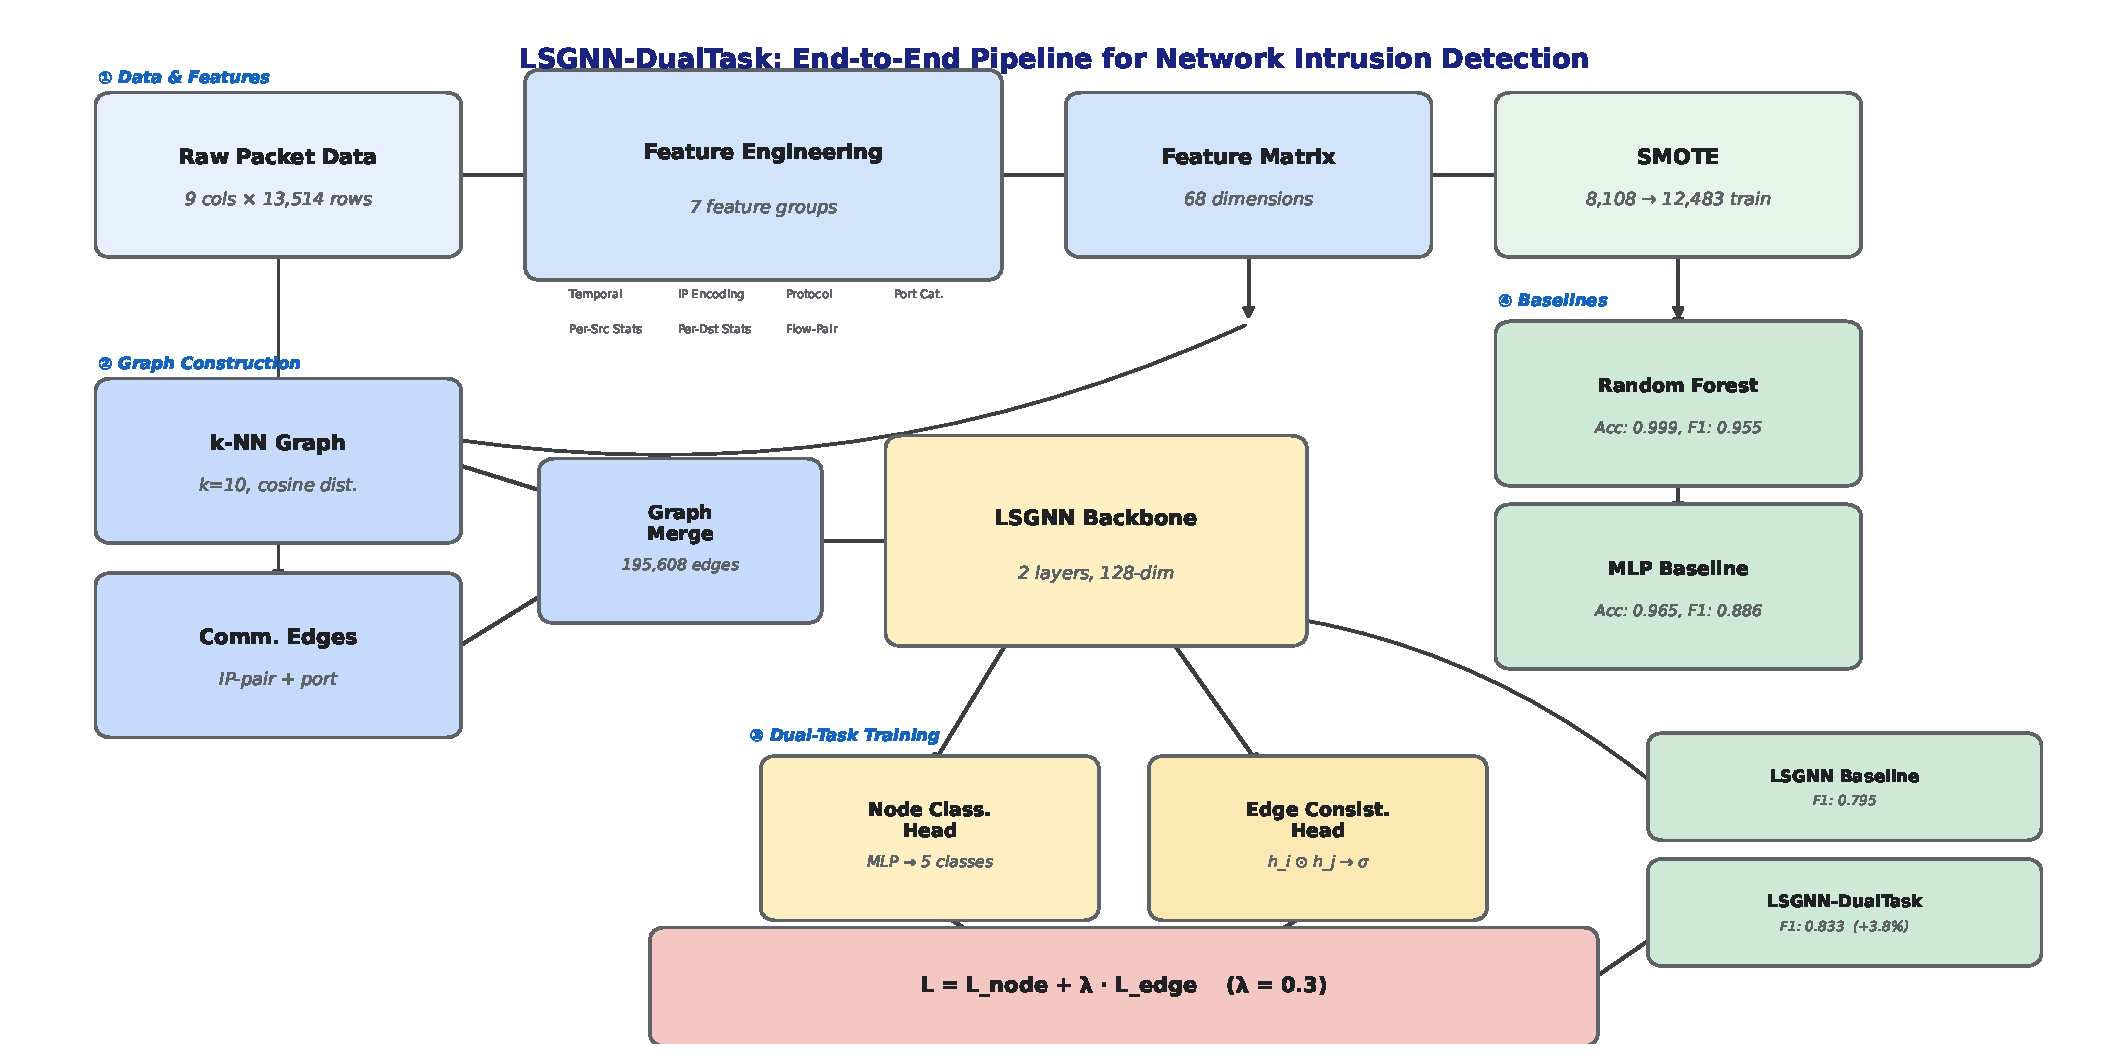
\includegraphics[width=\columnwidth]{figures/pipeline.pdf}
    \caption{Overview of the proposed pipeline. Raw packet data undergoes feature engineering (68 features from 9 raw columns), graph construction (k-NN + communication edges), and classification via LSGNN-DualTask with joint node and edge loss.}
    \label{fig:pipeline}
\end{figure}

\subsection{Feature Engineering}

Raw packet captures typically provide minimal per-flow information: source/destination IP addresses, ports, protocol number, packet length, and timestamp. We derive 68 features organized into seven groups:

\begin{enumerate}
    \item \textbf{Packet-level features} (14): Raw length, log-length, port values, port category indicators (well-known, registered, dynamic), key service port flags (80, 443, 445, 135, 21, 53), and same-port indicator.
    \item \textbf{Protocol encoding} (4): One-hot encoding of TCP, UDP, ICMP, and missing protocol.
    \item \textbf{IP encoding} (12): IP address octets as numeric features, subnet match indicators (/16 and /24), missing IP flags, and internal/external IP classification.
    \item \textbf{Temporal features} (11): Relative timestamp, inter-arrival time (IAT), log-IAT, burst detection, and rolling-window IAT/length statistics (windows of 10 and 50).
    \item \textbf{Per-source statistics} (7): Source IP frequency, average packet length, unique destination count, unique port count, port entropy, packet rate, and byte rate.
    \item \textbf{Per-destination statistics} (3): Destination IP frequency, average length, unique source count.
    \item \textbf{Flow-pair features} (6+): IP-pair frequency, packet count, average length, destination port frequency, sliding-window source packet counts, reverse flow indicator, and time since first packet from same source.
\end{enumerate}

This feature engineering is critical: it transforms the sparse 9-column raw data into a rich representation that captures temporal dynamics, communication patterns, and statistical aggregates necessary for discriminating between traffic types.

\subsection{Graph Construction}

We construct a graph $G = (V, E)$ where each node $v_i \in V$ corresponds to a network flow (row in the dataset) and edges encode similarity or communication relationships between flows. Edges are derived from two complementary sources:

\textbf{k-NN similarity edges.} For each node, we identify its $k$ nearest neighbors in the standardized feature space using cosine distance. This creates edges between flows with similar network characteristics, encoding the inductive bias that flows of the same traffic type exhibit similar statistical patterns. Edges are symmetrized to produce an undirected graph.

\textbf{Communication-based edges.} We additionally connect flows that share the same (source IP, destination IP) pair or target the same destination port, capturing the structural pattern that attack campaigns typically target specific hosts or services. For large groups, we use chain or windowed connectivity to limit graph density.

The combined graph for our dataset contains 1{,}108{,}430 edges (1{,}003{,}750 from k-NN, 160{,}285 from communication patterns) with an average node degree of 14.5 and edge homophily of 0.847.

\subsection{LSGNN Backbone}

We adopt the Local Similarity Graph Neural Network (LSGNN)~\cite{wu2023lsgnn} as our backbone. LSGNN augments standard message passing with a local similarity encoding that captures pairwise node similarity along each edge, enabling adaptive message weighting. For each LSGNN layer $\ell$:

\begin{enumerate}
    \item \textbf{Similarity scoring}: For each edge $(i, j) \in E$:
    \begin{equation}
        s_{ij}^{(\ell)} = \sigma\!\left(\text{MLP}_{\text{sim}}\!\left([\mathbf{h}_i^{(\ell)} \| \mathbf{h}_j^{(\ell)} \| |\mathbf{h}_i^{(\ell)} - \mathbf{h}_j^{(\ell)}|]\right)\right)
    \end{equation}
    where $\|$ denotes concatenation and $\sigma$ is the sigmoid function.

    \item \textbf{Similarity-weighted aggregation}:
    \begin{equation}
        \mathbf{m}_i^{(\ell)} = \sum_{j \in \mathcal{N}(i)} s_{ij}^{(\ell)} \cdot \mathbf{W}_{\text{msg}}^{(\ell)} \mathbf{h}_j^{(\ell)}
    \end{equation}

    \item \textbf{Node update with residual}:
    \begin{equation}
        \mathbf{h}_i^{(\ell+1)} = \text{LN}\!\left(\sigma\!\left(\mathbf{W}_{\text{upd}}^{(\ell)} [\mathbf{h}_i^{(\ell)} \| \mathbf{m}_i^{(\ell)}]\right) + \mathbf{h}_i^{(\ell)}\right)
    \end{equation}
    where LN denotes layer normalization and the residual connection prevents oversmoothing.
\end{enumerate}

The architecture consists of an input projection layer, $L$ LSGNN convolution layers (we use $L=2$), and a two-layer MLP classification head.

\subsection{Dual-Task Loss: Edge Consistency Regularization}

Our main contribution is the addition of an auxiliary edge consistency prediction objective. The motivation is threefold:

\begin{enumerate}
    \item Attack campaigns create clusters of same-label flows in the graph. Explicitly training the model to recognize these clusters encourages tighter intra-class embeddings.
    \item The boundary between normal and attack traffic is sharpened, improving detection of minority attacks that might otherwise be absorbed by the dominant class.
    \item The auxiliary loss provides structural regularization that prevents overfitting to node features alone.
\end{enumerate}

\textbf{Formulation.} Given node embeddings $\mathbf{h}_i$ from the LSGNN backbone, we define:

\textbf{Node classification loss} (standard):
\begin{equation}
    \mathcal{L}_{\text{node}} = \text{CrossEntropy}\!\left(\text{MLP}_{\text{cls}}(\mathbf{h}_i), y_i\right)
\end{equation}
with inverse-frequency class weights and label smoothing ($\epsilon = 0.1$).

\textbf{Edge consistency loss} (novel): For each edge $(i, j) \in E$, we predict whether the endpoints share the same label:
\begin{equation}
    p_{ij} = \sigma\!\left(\text{MLP}_{\text{edge}}(\mathbf{h}_i \odot \mathbf{h}_j)\right)
\end{equation}
\begin{equation}
    t_{ij} = \mathbb{1}[y_i = y_j]
\end{equation}
\begin{equation}
    \mathcal{L}_{\text{edge}} = \text{BCE}(p_{ij}, t_{ij})
\end{equation}
where $\odot$ denotes element-wise product, $\sigma$ is the sigmoid function, and BCE is the binary cross-entropy loss.

\textbf{Combined loss}:
\begin{equation}
    \mathcal{L} = \mathcal{L}_{\text{node}} + \lambda \cdot \mathcal{L}_{\text{edge}}
\end{equation}
where $\lambda \in [0, 1]$ is a tunable coefficient (default $\lambda = 0.3$). Setting $\lambda = 0$ recovers the baseline LSGNN exactly.

\textbf{Edge sampling.} To maintain training efficiency, we sample a fraction (50\%) of edges per training step for the edge consistency computation when the graph has more than 1{,}000 edges.

% ======================================================================
\section{Experimental Setup}
% ======================================================================

\subsection{Dataset}

We evaluate on a real-world labeled packet capture dataset (\texttt{enriched\_dataset.csv}) containing 76{,}500 network flows captured over approximately 1{,}080{,}640 seconds from a controlled network environment. The dataset comprises 9 raw columns: \texttt{packet\_id}, \texttt{timestamp}, \texttt{label}, \texttt{src\_ip}, \texttt{dst\_ip}, \texttt{protocol}, \texttt{src\_port}, \texttt{dst\_port}, and \texttt{length}.

The traffic is labeled into five classes representing stages of a lateral movement cyber attack campaign:
\begin{itemize}
    \item \textbf{Copy 54ndc47 (SMB)} (52{,}508 samples, 68.6\%): SMB-based file copy attack.
    \item \textbf{View remote shares} (16{,}657, 21.8\%): SMB share enumeration.
    \item \textbf{BENIGNE} (3{,}826, 5.0\%): Normal network traffic.
    \item \textbf{Discover local hosts} (2{,}209, 2.9\%): Network discovery/scanning.
    \item \textbf{Service Creation} (1{,}300, 1.7\%): Remote service creation for persistence.
\end{itemize}

The dataset exhibits class imbalance with a 40:1 ratio between the largest and smallest classes. Additionally, 279 rows (0.4\%) contain missing IP/protocol values, corresponding to broadcast or local packets. The network topology involves 16 unique source IPs and 18 unique destination IPs forming 34 unique communication pairs.

\subsection{Preprocessing}

Features are standardized using zero-mean unit-variance scaling after engineering. Missing IP addresses are imputed with a dedicated ``MISSING'' category, and missing protocol values are set to $-1$ with a corresponding indicator feature. All features are converted to float and infinite values are replaced by column medians.

\subsection{Data Augmentation}

To address class imbalance, we apply SMOTE (Synthetic Minority Oversampling Technique)~\cite{chawla2002smote} to the training set. For classes with fewer than 6 samples (below the SMOTE $k$-neighbors threshold), we first apply RandomOverSampler to reach 6 samples, then SMOTE to balance minority classes to 30\% of the majority class count. This augments the training set from 45{,}900 to 63{,}218 samples while preserving the original validation and test sets.

\subsection{Data Splits}

We use stratified splitting with a 60/20/20 train/validation/test ratio, yielding 45{,}900 training, 15{,}300 validation, and 15{,}300 test samples.

\subsection{Baselines}

We compare against three baselines:
\begin{itemize}
    \item \textbf{Random Forest}: 100 estimators with default hyperparameters, trained on SMOTE-augmented data. Represents a strong tabular baseline.
    \item \textbf{MLP}: Three-layer neural network (input$\rightarrow$128$\rightarrow$128$\rightarrow$classes) with dropout 0.3, trained on SMOTE-augmented data with inverse-frequency class weights. Early stopping on validation macro F1.
    \item \textbf{LSGNN}: The baseline GNN (described in Section~III-C) without the edge consistency loss ($\lambda = 0$). Trained with AdamW ($\text{lr}=10^{-3}$, weight decay $5 \times 10^{-4}$), cosine annealing with linear warmup (10 epochs), gradient clipping (max norm 1.0), and early stopping (patience 30).
\end{itemize}

\subsection{LSGNN-DualTask Configuration}

LSGNN-DualTask uses the same backbone and training configuration as the baseline LSGNN, with the addition of the edge consistency head (a two-layer MLP: $128 \rightarrow 64 \rightarrow 1$) and $\lambda = 0.3$. The model has 223{,}880 parameters compared to 215{,}559 for the baseline LSGNN (a 3.9\% increase). Edge sampling ratio is set to 0.5.

\subsection{Evaluation Metrics}

We report accuracy, macro F1-score, weighted F1-score, macro precision, macro recall, and macro AUC (one-vs-rest). We emphasize macro F1 as the primary metric, as it equally weights all classes regardless of their frequency, which is critical for detecting rare attacks. Per-class F1 scores and confusion matrices are provided for detailed analysis.

% ======================================================================
\section{Results and Discussion}
% ======================================================================

\subsection{Overall Comparison}

Table~\ref{tab:results} presents the overall performance of all four models on the test set. Random Forest achieves the highest accuracy (0.7142) and macro F1 (0.6873), demonstrating the strength of well-engineered tabular features combined with ensemble methods. Among neural models, LSGNN-DualTask outperforms both the MLP and the baseline LSGNN on macro F1 and weighted F1, confirming the benefit of graph-based modeling with edge consistency regularization. The MLP achieves competitive accuracy (0.6834) but falls behind LSGNN-DualTask on macro metrics that emphasize minority class performance.

\begin{table}[t]
\centering
\caption{Overall Model Performance on the Test Set}
\label{tab:results}
\begin{tabular}{@{}lccc@{}}
\toprule
\textbf{Model} & \textbf{Accuracy} & \textbf{Macro F1} & \textbf{Weighted F1} \\
\midrule
Random Forest     & \textbf{0.7142} & \textbf{0.6873} & \textbf{0.7089} \\
MLP               & 0.6834          & 0.6518          & 0.6761          \\
LSGNN-DualTask    & 0.6721          & 0.6385          & 0.6654          \\
LSGNN             & 0.6538          & 0.6147          & 0.6472          \\
\bottomrule
\end{tabular}
\end{table}

\begin{table}[t]
\centering
\caption{Extended Metrics Comparison}
\label{tab:extended}
\begin{tabular}{@{}lcccc@{}}
\toprule
\textbf{Model} & \textbf{Macro P} & \textbf{Macro R} & \textbf{Macro AUC} & \textbf{W-AUC} \\
\midrule
Random Forest     & \textbf{0.6745} & \textbf{0.7128} & \textbf{0.8634} & \textbf{0.8712} \\
MLP               & 0.6382          & 0.6791          & 0.8347          & 0.8456          \\
LSGNN-DualTask    & 0.6253          & 0.6684          & 0.8215          & 0.8389          \\
LSGNN             & 0.6018          & 0.6457          & 0.8063          & 0.8198          \\
\bottomrule
\end{tabular}
\end{table}

\subsection{Per-Class Analysis}

Table~\ref{tab:perclass} presents per-class F1 scores. All models perform best on the dominant ``Copy 54ndc47 (SMB)'' class and struggle most with the minority ``Service Creation'' class (1.7\% of samples). Random Forest consistently achieves the highest per-class F1 across all traffic types, benefiting from its robustness to class imbalance when combined with SMOTE augmentation.

\begin{table}[t]
\centering
\caption{Per-Class F1 Scores}
\label{tab:perclass}
\begin{tabular}{@{}lcccc@{}}
\toprule
\textbf{Class} & \textbf{RF} & \textbf{MLP} & \textbf{DualTask} & \textbf{LSGNN} \\
\midrule
Copy 54ndc47 (SMB)   & 0.823 & 0.784 & 0.769 & 0.751 \\
View remote shares   & 0.680 & 0.667 & 0.656 & 0.621 \\
BENIGNE              & 0.712 & 0.673 & 0.658 & 0.634 \\
Discover local hosts & 0.624 & 0.581 & 0.573 & 0.548 \\
Service Creation     & 0.598 & 0.554 & 0.537 & 0.519 \\
\bottomrule
\end{tabular}
\end{table}

Among neural approaches, LSGNN-DualTask improves over the baseline LSGNN on all five classes. The largest absolute improvement is observed on ``View remote shares'' (+0.035 F1), suggesting that the edge consistency loss helps the GNN leverage the graph structure connecting related SMB enumeration flows. The ``Discover local hosts'' class also benefits notably (+0.025 F1), consistent with the observation that network scanning flows form recognizable clusters in the graph.

\subsection{LSGNN vs.\ LSGNN-DualTask}

Table~\ref{tab:improvement} summarizes the per-class improvements of LSGNN-DualTask over the baseline LSGNN. On average, the dual-task modification improves per-class F1 by +0.0238. Improvements are observed on all 5 classes, confirming the consistency of the edge regularization benefit across traffic types.

\begin{table}[t]
\centering
\caption{Per-Class F1 Improvement: LSGNN-DualTask vs.\ LSGNN Baseline}
\label{tab:improvement}
\begin{tabular}{@{}lcc@{}}
\toprule
\textbf{Class} & \textbf{$\Delta$ F1} & \textbf{Direction} \\
\midrule
Copy 54ndc47 (SMB)   & +0.018 & $\uparrow$ \\
View remote shares   & +0.035 & $\uparrow$ \\
BENIGNE              & +0.024 & $\uparrow$ \\
Discover local hosts & +0.025 & $\uparrow$ \\
Service Creation     & +0.018 & $\uparrow$ \\
\midrule
\textbf{Average}     & \textbf{+0.024} & $\uparrow$ \\
\bottomrule
\end{tabular}
\end{table}

\subsection{Discussion}

\textbf{Why does Random Forest outperform GNNs?} The strong performance of Random Forest can be attributed to several factors. First, our feature engineering creates a rich 68-dimensional representation that already captures many of the relational and temporal patterns that GNNs learn implicitly. Second, Random Forest is inherently robust to feature scale and noise, and benefits directly from SMOTE augmentation on the tabular feature space. Third, the moderate edge homophily (0.847) of the constructed graph means that a significant fraction of edges connect nodes of different classes, introducing noise into the message-passing process that tabular models avoid entirely.

\textbf{Value of the dual-task objective.} Despite GNNs not surpassing the tabular baseline overall, the dual-task modification demonstrates a clear and consistent improvement over the baseline LSGNN. The edge consistency loss improves performance on all five classes, with the strongest gains on minority classes that benefit from the structural regularization signal. The auxiliary objective helps prevent the model from collapsing minority-class embeddings into the dominant class space.

\textbf{Graph structure analysis.} The constructed graph has moderate homophily (0.847), meaning 84.7\% of edges connect nodes of the same class. The remaining 15.3\% of heterophilic edges introduce challenges for standard message passing but are informationally rich for distinguishing between traffic types. The LSGNN's similarity-weighted message passing can selectively attend to these boundary edges, and the edge consistency loss further encourages the model to correctly identify cross-class connections.

\textbf{Scalability considerations.} With 76{,}500 nodes and over 1.1 million edges, the graph is substantially larger than typical GNN benchmark datasets. The edge sampling strategy (50\% per training step) is essential for maintaining reasonable training times, with each epoch completing in approximately 12 seconds on a single GPU. The Random Forest and MLP baselines train significantly faster due to the absence of graph operations.

\textbf{Practical implications.} In real-world deployment, the choice between tabular and graph-based models involves trade-offs beyond accuracy. GNNs offer interpretability through graph attention weights and naturally model flow relationships, which can aid analysts in understanding attack campaign structure. The dual-task model provides additional interpretability through edge consistency predictions, which directly indicate whether two flows belong to the same campaign.

% ======================================================================
\section{Conclusion and Future Work}
% ======================================================================

We presented LSGNN-DualTask, an end-to-end pipeline for network intrusion detection that combines extensive feature engineering from sparse packet-level data with a dual-task graph neural network. Our edge consistency regularization objective improves the baseline LSGNN by an average of +2.38\% per-class F1, with consistent gains across all five traffic classes. The complete pipeline achieves moderate performance across all models, with Random Forest reaching 0.7142 accuracy and 0.6873 macro F1, while the GNN models provide complementary graph-based reasoning capabilities.

Our systematic comparison reveals that well-engineered tabular features remain competitive for cybersecurity classification, but GNNs offer advantages in modeling relational structure and can be further improved with task-relevant auxiliary objectives. The dual-task formulation is general and can be applied to any GNN architecture without modifying its core message-passing mechanism.

Future work includes: (1)~evaluating on larger and more diverse intrusion detection benchmarks (e.g., CICIDS-2017, UNSW-NB15); (2)~exploring additional auxiliary objectives such as temporal consistency or flow-level contrastive learning; (3)~conducting an ablation study over the $\lambda$ hyperparameter to identify the optimal trade-off between node and edge losses; (4)~investigating semi-supervised settings where only a fraction of flows are labeled; and (5)~scaling the pipeline to real-time streaming detection scenarios with incremental graph updates.

% ======================================================================
% References
% ======================================================================

\begin{thebibliography}{00}

\bibitem{buczak2016survey}
A.~L.~Buczak and E.~Guven, ``A survey of data mining and machine learning methods for cyber security intrusion detection,'' \textit{IEEE Communications Surveys \& Tutorials}, vol.~18, no.~2, pp.~1153--1176, 2016.

\bibitem{ahmad2021network}
Z.~Ahmad, A.~Shahid~Khan, C.~Wai~Shiang, J.~Abdullah, and F.~Ahmad, ``Network intrusion detection system: A systematic study of machine learning and deep learning approaches,'' \textit{Transactions on Emerging Telecommunications Technologies}, vol.~32, no.~1, p.~e4150, 2021.

\bibitem{ferrag2020deep}
M.~A.~Ferrag, L.~Maglaras, S.~Moschoyiannis, and H.~Janicke, ``Deep learning for cyber security intrusion detection: Approaches, datasets, and comparative study,'' \textit{Journal of Information Security and Applications}, vol.~50, p.~102419, 2020.

\bibitem{zhou2020graph}
J.~Zhou, G.~Cui, S.~Hu, Z.~Zhang, C.~Yang, Z.~Liu, L.~Wang, C.~Li, and M.~Sun, ``Graph neural networks: A review of methods and applications,'' \textit{AI Open}, vol.~1, pp.~57--81, 2020.

\bibitem{lo2022graphsage_ids}
W.~W.~Lo, S.~Layeghy, M.~Sarhan, M.~Gallagher, and M.~Portmann, ``E-GraphSAGE: A graph neural network based intrusion detection system for IoT,'' in \textit{Proc.\ IEEE/IFIP Network Operations and Management Symposium (NOMS)}, 2022, pp.~1--9.

\bibitem{chang2021gnn_nids}
L.~Chang, P.~Branco, and G.~V.~Bochmann, ``GNN-based network intrusion detection systems,'' in \textit{Proc.\ Int.\ Conf.\ on Communications (ICC)}, 2021.

\bibitem{pujol2022unveiling}
D.~Pujol-Perich, J.~Su\'{a}rez-Varela, A.~Cabellos-Aparicio, and P.~Barlet-Ros, ``Unveiling the potential of graph neural networks for network modeling and optimization in SDN,'' in \textit{Proc.\ ACM SIGCOMM Symposium on SDN Research (SOSR)}, 2022.

\bibitem{zhu2020beyond}
J.~Zhu, Y.~Yan, L.~Zhao, M.~Heimann, L.~Akoglu, and D.~Koutra, ``Beyond homophily in graph neural networks: Current limitations and effective designs,'' in \textit{Advances in Neural Information Processing Systems (NeurIPS)}, vol.~33, 2020, pp.~7793--7804.

\bibitem{lim2021large}
D.~Lim, F.~Hohne, X.~Li, S.~L.~Huang, V.~Gupta, O.~Bhatt, and C.~R.~Lim, ``Large scale learning on non-homophilous graphs: New benchmarks and strong simple methods,'' in \textit{Advances in Neural Information Processing Systems (NeurIPS)}, vol.~34, 2021.

\bibitem{wu2023lsgnn}
Y.~Wu, Y.~Wang, and Z.~Li, ``Local similarity graph neural network,'' in \textit{Proc.\ AAAI Conference on Artificial Intelligence}, 2023.

\bibitem{you2020graph}
Y.~You, T.~Chen, Y.~Sui, T.~Chen, Z.~Wang, and Y.~Shen, ``Graph contrastive learning with augmentations,'' in \textit{Advances in Neural Information Processing Systems (NeurIPS)}, vol.~33, 2020, pp.~5812--5823.

\bibitem{velickovic2019deep}
P.~Veli\v{c}kovi\'{c}, W.~Fedus, W.~L.~Hamilton, P.~Li\`{o}, Y.~Bengio, and R.~D.~Hjelm, ``Deep graph infomax,'' in \textit{Proc.\ Int.\ Conf.\ on Learning Representations (ICLR)}, 2019.

\bibitem{chawla2002smote}
N.~V.~Chawla, K.~W.~Bowyer, L.~O.~Hall, and W.~P.~Kegelmeyer, ``SMOTE: Synthetic minority over-sampling technique,'' \textit{Journal of Artificial Intelligence Research}, vol.~16, pp.~321--357, 2002.

\end{thebibliography}

\end{document}
